\sectioncounter{10}
  \section{幂函数, 函数与方程}

  \subsection{知识梳理}
  形如 $y=x^a$ 的函数称为\myindex{幂函数} (power function). 应注意: 幂函数的底为自变量, 指数不变, 
  而指数函数的底不变, 指数为自变量. 考虑 $f(x)=x^2$, $g(x)=x^{\frac12}$ 
  和 $h(x)=x^{-1}$ 的图象 (如图~\ref{fig-190216-2250}) 可知, 
  幂函数 $y=x^a$ 恒过点~$(1,1)$, 且在第一象限, 
  当 $a<0$ 时函数单调减少, 当 $a>0$ 时函数单调增加.
  \begin{figure}[htb]
    \centering\small
    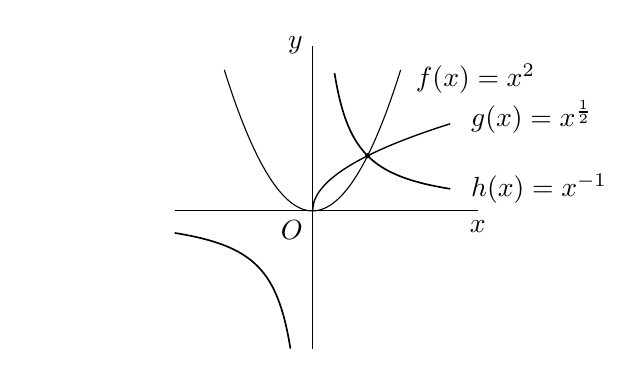
\begin{tikzpicture}[scale=0.7]
      \draw[\myaxisarrow] (-2.5,0) -- (3,0) node[below] {$x$};
      \draw[\myaxisarrow] (0,-2.5) -- (0,3) node[left] {$y$};
      \draw[line width=0.6pt,smooth,samples=100]
        plot[domain=0.4:2.5](\x,{1/\x})
        plot[domain=-2.5:-0.4](\x,{1/\x});
      \draw[line width=0.5pt,smooth,samples=100,domain=0:2.5] plot(\x,{sqrt(\x)});
      \draw[line width=0.4pt,smooth,samples=100,domain=-1.6:1.6] plot(\x,{(\x)^2});
      
      \draw [fill=black] (1,1) circle (1pt);
      \draw (0,0) node[anchor=north east] {$O$};
      \draw (1.7,2.4) node[right] {$f(x)=x^2$};
      \draw (2.7,1.7) node[right] {$g(x)=x^{\frac12}$};
      \draw (2.7,0.4) node[right] {$h(x)=x^{-1}$};
      \draw (-5,0) node {};
    \end{tikzpicture}
    \caption{}\label{fig-190216-2250}
  \end{figure}

  求方程的根可以转化为求对应函数图象交点的横坐标, 或求对应函数的零点. 
  一般有如下两种转化方法:
  \begin{align*}
    f(x)=0\text{\ 的根}&\Leftrightarrow 
      \text{$f(x)$ 的图象与 $x$ 轴交点的横坐标};\\
    f(x)+g(x)=0\text{\ 的根}&\Leftrightarrow 
      \text{$f(x)$ 与 $-g(x)$ 的图象交点的横坐标}.
  \end{align*}
  前一种方法可视为后一种方法的特例, 而两种方法在使用时都需要考虑函数的单调性.
  此外还有
  
  \myemph{零点存在性定理}: 若 $f(x)$ 在 $[a,b]$ 上连续, 且 $f(a)f(b)<0$, 
  则 $f(x)$ 在 $(a,b)$ 上至少有一根. 
  
  如果只求方程的根的个数, 通常作出对应函数的大致图象即可. 但若求方程的根的取值范围, 则需要适当计算函数值并利用零点存在性定理判断根的存在区间.

  \lianxi
  \begin{exercise}
    幂函数的图象不过第 $\underline{\qquad}$ 象限.
  \end{exercise}

  \beginsolution
    ``四''.
  \endsolution
  
  \begin{exercise}
    已知幂函数 $y=x^\alpha$ 的图象过点 $\Big(3, \frac19\Big)$,
    求它的单调增区间.
  \end{exercise}

  \beginsolution
    $\frac19=3^\alpha$, $\alpha=-2$, 则 $y=x^{-2}$, 单调递增区间为 $(-\infty,0)$.
  \endsolution
  
  \begin{exercise}
    若函数 $f(x)=x^2 -ax-b$ 的两个零点是 $2$ 和 $3$, 
    则函数 $g(x)=bx^2 -ax-1$ 的零点是\,?
  \end{exercise}

  \beginsolution
    由韦达定理, $a=2+3$, $-b=2\cdot 3$, 
    \mymarginpar{由已知也可直接得到 
      \[f(x)=(x-2)(x-3).\]}
    即 $a=5$, $b=-6$, 所以 $g(x)=-6x^2-5x-1$, 零点为 $-\frac12$, $-\frac13$.
  \endsolution
  
  \begin{exercise}
    解方程: $\mathrm{e}^x+x=1$.
  \end{exercise}

  \beginsolution
    方法一: 设 $f(x)=\mathrm{e}^x+x$, 则 $f(x)$ 在 $\mathbb{R}$ 上 $\nearrow$ 且 $f(0)=1$, 所以方程只有唯一的根 $x=0$.
    
    方法二: 方程化为 $\mathrm{e}^x=1-x$, 作对应函数图象知, $x=1$.
  \endsolution
  
  \subsection{要点导学\quad 各个击破}
  \subsubsection{幂函数的图象与性质}
  \begin{example}
    设 $a=2^{0.3}$, $b=3^{0.2}$, $c=7^{0.1}$, 则 $a$, $b$, $c$ 
    的大小关系为\,?
  \end{example}

  \beginsolution
    $a^{10}=2^3=8$, $b^{10}=3^2=9$, $c^{10}=7$, 所以 $c^{10}<a^{10}<b^{10}$, 即 $c<a<b$.
  \endsolution
  
  \lianxi
  \begin{exercise}[s]
    若幂函数 $f(x)=x^\alpha$ 的图象过点 $(2,4)$, 求函数 $f(x)$ 的单调递增区间.
  \end{exercise}

  \beginsolution
    $2^\alpha=4$, $\alpha=2$, $f(x)=x^2$, 单调递增区间为 $[0,+\infty)$.
  \endsolution
  
  \subsubsection{求函数的零点}
  \begin{example}
    已知 $f(x)$ 是定义在 $\mathbb{R}$ 上的奇函数, 
    当 $x\geqslant 0$ 时, $f(x)=x^2 -3x$, 
    求函数 $g(x)=f(x)-x+3$ 的零点集.
  \end{example}

  \beginsolution
    方法一: 若 $x\geqslant 0$, 则 $g(x)=x^2-4x+3=0$, 解得 $x=1$, $3$.
    若 $x<0$, 则 $-x>0$, $f(x)=-f(-x)=-x^2-3x$, $g(x)=-x^2-4x+3=0$, 解得 $x=-2\pm\sqrt7$, 取 $x=-2-\sqrt7$. 综上所述, $g(x)$ 的零点集为 $\{-2-\sqrt7, 1, 3\}$.
    
    方法二: 也可利用 $f(x)$ 为奇函数, 作图找 $f(x)=x-3$ 的零点.
  \endsolution
  
  \begin{example}
    根据表格中的数据, 可以判定方程 $\mathrm{e}^x -x-2=0$ 
    的一个根所在的区间为 $(k,k+1)$ ($k\in \mathbb{Z}$),
    求 $k$ 的值.
    \begin{center}
    \small
    \begin{tabular}{cccccc}
      \toprule
      $x$ & $-1$ & $0$ & $1$ & $2$ & $3$\\
      \midrule
      $\mathrm{e}^x$ & $0.37$ & $1$ & $2.72$ & $7.39$ & $20.09$\\
      $x+2$ & $1$ & $2$ & $3$ & $4$ & $5$ \\
      \bottomrule
    \end{tabular}
    \end{center}
  \end{example}

  \beginsolution
    由零点存在性定理知, 区间 $(1,2)$ 之中至少有一根, 故 $k=1$.
    
    \varexercise 若方程 $\mathrm{e}^x -x-2=0$ 的根所在区间为 $(k,k+1)$ ($k\in \mathbb{Z}$), 求 $k$ 的值.
    
    设 $f(x)=\mathrm{e}^x -x-2$, 则 $f'(x)=\mathrm{e}^x-1$, 可知 $f(x)$ 在 $(-\infty,0)$ 上 $\searrow$, 在 $(0,+\infty)$ 上 $\nearrow$. 而
    \begin{align*}
      f(-2)= \mathrm{e}^{-2}>0,&\quad f(-1)=\mathrm{e}^{-1}-1<0,\\
      f(1)=\mathrm{e}-3<0,&\quad f(2)=\mathrm{e}^2-4>0,
    \end{align*}
    所以 $f(x)=0$ 只有两个根且分别在区间 $(-2,-1)$ 和 $(1,2)$ 内, 即 $k=-2$ 或 $1$. (此题也可把方程化为 $\mathrm{e}^x=x+2$, 利用函数图象结合估值, 得到根的大致区间.)
    
    \varexercise 若方程 $\mathrm{e}^x -x-2=0$ 的根所在区间为 $\Big(\frac{k}2,\frac{k+1}2\Big)$ ($k\in \mathbb{Z}$), 求 $k$ 的值.
    
    由
    \mymarginpar{不断地把一根所在区间二等分, 比较分点处函数值与 $0$ 的大小, 就可以得到根更精确的取值区间. 这种方法叫做\myemph{二分法}.}
    \begin{gather*}
      f(-2)>0,\quad f\Bigl(-\frac32\Bigr)=\mathrm{e}^{-\frac32}-\frac12<0,\\
      f(1)<0,\quad f\Big(\frac32\Big)=\mathrm{e}^{\frac32}-\frac72>0,
    \end{gather*}
    知 $f(x)=0$ 的两个根分别在区间 $\Bigl(-2,-\frac32\Bigr)$ 和 $\Big(1,\frac32\Big)$ 内, 即 $k=-4$ 或 $2$.
  \endsolution
  
  \lianxi
  \begin{exercise}
    设函数 $f(x)=x^3$ 与 $g(x)=\Big(\frac12\Big)^{x-2}$ 的图象的交点为
    $(x_0,y_0)$, 且 $x_0 \in (m,m+1)$, $m\in \mathbb{Z}$, 
    求 $m$ 的值.
  \end{exercise}

  \beginsolution
    作 $f(x)$ 和 $g(x)$ 的大致图象知, $x_0>0$. 由
    \mymarginpar{估计根所在范围时, 图象法可确定大致范围, 而计算法可确定较精确的范围.}
    \[f(1)-g(1)=-1<0,\quad f(2)-g(2)=7>0\]
    知 $x_0\in(1,2)$, 则 $m=1$.
    
    \varexercise 若 $x_0\in\Big(\frac{m}2,\frac{m+1}2\Big)$, $m\in\mathbb{Z}$, 其余条件不变, 求 $m$ 的值.
    
    由
    \[f(1)-g(1)<0,\quad 
      f\Big(\frac32\Big)- g\Big(\frac32\Big)= \frac{27}8-2^{\frac12}\]
    知 $x_0\in\Big(1,\frac32\Big)$, 则 $m=2$.
  \endsolution
  
  \begin{exercise}
    判断方程 $x^2=2^x$ 的根的个数.
  \end{exercise}

  \beginsolution
    作 $f(x)=x^2$ 和 $g(x)=2^x$ 的图象知, 
    \mymarginpar{方程 $x^2=2^x$ 也可化为 $|x|=2^{\frac{x}2}$ 或 $2|t|=2^{t}$.}
    $x<0$ 时方程有一根在区间 $(-1,0)$ 内; $x\geqslant0$ 时有两根 $x=2$, $4$, 而此时方程可化为 $x=2^{\frac{x}2}$, 由函数图象知至多两根. 故 $x^2=2^x$ 共 $3$ 个根.
  \endsolution
  
  \subsubsection{函数零点的应用}
  \begin{example}
    设函数 $f(x)=\mathrm{e}^x +x-2$, $g(x)=\ln x+x^2-3$. 
    若实数 $a$,$b$ 满足 $f(a)=0$, $g(b)=0$, 
    则下列关系中正确的是\,?(填序号)
   
    (1) $g(a)<0<f(b)$;\qquad (2) $f(b)<0<g(a)$;
    
    (3) $0<g(a)<f(b)$;\qquad (4) $f(b)<g(a)<0$.
  \end{example}

  \beginsolution
    $f(x)$ 在 $\mathbb{R}$ 上 $\nearrow$, $g(x)$ 在区间 $(0,+\infty)$ 上 $\nearrow$, 则由
    \mymarginpar{应充分利用函数的单调性估计根的取值范围.}
    \begin{gather*}
      f(0)=-1<0,\quad f(1)=\mathrm{e}-1>0,\\
      g(1)=-2<0,\quad g(2)=\ln2+1>0
    \end{gather*}
    知 $0<a<1<b<2$, 故
    \[g(a)<g(1)<0<f(1)<f(b),\]
    选 ``(1)''.
  \endsolution
  
  \subsubsection{函数与方程的关系}
  \begin{example}
    设函数 $f(x)=\begin{cases}
      x^2+bx+c, & x\leqslant 0,\\
      2, & x>0.\end{cases}$ 若 $f(-4)=f(0)$, $f(-2)=-2$, 
    求关于 $x$ 的方程 $f(x)=x$ 的根的个数.
  \end{example}

  \beginsolution
    由 $f(-4)=f(0)$ 知二次函数图象的轴为 $x=-2$, 故 $f(-2)=-2$ 表明 $x\leqslant 0$ 时, $f(x)=(x+2)^2-2$. 关于 $x$ 分类讨论解 $f(x)=x$ 得, $x=-1$, $\pm2$, 共 $3$ 个根.
  \endsolution
  
  \lianxi
  \begin{exercise}[s]
    已知函数 $f(x)=ax^2 +4x+b$ ($a\neq0$), 且方程 $f(x)=x$ 的两实根为 $\alpha$,$\beta$. 若 $|\alpha-\beta|=1$, 求 $a$, $b$ 之间的函数关系式.
  \end{exercise}

  \beginsolution
    $f(x)=x$ 化为 $ax^2+3x+b=0$, 则 
    \[|\alpha-\beta|= \frac{\sqrt{9-4ab}}{|a|}=1, \text{\ 即 }
      b=\frac{9-a^2}{4a}.\]
  \endsolution
  
  \subsubsection{课堂评价}
  \begin{exercise}
    对于函数 $y=x^2$, $y=x^{\frac12}$, 下列说法中正确的是?
    
    (1) 两个函数都是幂函数;\qquad
    (2) 两个函数在 $(0,+\infty)$ 上都单调递增;
    
    (3) 两个函数的图象关于直线 $y=x$ 对称;\qquad
    (4) 两个函数都是偶函数.
  \end{exercise}

  \beginsolution
    选 ``(1)'' 和 ``(2)''.
  \endsolution
  
  \begin{exercise}
    在下列区间中, 函数 $f(x)=\mathrm{e}^x +4x-3$ 
    的零点所在的区间是\,?
    
    (1) $\Big(0,\frac14\Big)$;\qquad
    (2) $\Big(\frac14,\frac12\Big)$;\qquad
    (3) $\Big(\frac12,\frac34\Big)$;\qquad
    (4) $\Big(\frac34,1\Big)$.
  \end{exercise}

  \beginsolution
    $f(x)$ 在 $\mathbb{R}$ 上 $\nearrow$, 且 
    \[f\Big(\frac14\Big)=\mathrm{e}^{\frac14}-2<0,\quad
      f\Big(\frac12\Big)=\mathrm{e}^{\frac12}-1<0,\]
    故选 ``(2)''.
  \endsolution
  
  \begin{exercise}
    若 $f(x)=\ln x+x-2$ 零点所在区间是 $(k,k+1)$ ($k\in\mathbb{Z}$),
    求 $k$ 的值.
  \end{exercise}

  \beginsolution
    $f(x)$ 在 $(0,+\infty)$ 上 $\nearrow$, $f(1)=-1<0$, $f(2)=\ln2>0$, 故 $k=1$.
  \endsolution
  
  \subsection{课后练习}
  \begin{exercise}
    设 $\alpha\in \Bigl\{-1,1,\frac12,3\Bigr\}$, 
    则使函数 $y=x^\alpha$ 的定义域为 $\mathbb{R}$ 
    且为奇函数的所有 $\alpha$ 的值为\,?
  \end{exercise}

  \beginsolution
    $\alpha=1$,$3$.
  \endsolution
  
  \begin{exercise}
    设 $f(x)=\mathrm{e}^x -2x-2$ 零点所在区间为 $(k,k+1)$ 
    ($k\in\mathbb{Z}$), 则 $k=$\,?
  \end{exercise}

  \beginsolution
    $f'(x)=\mathrm{e}^x-2$, 则 $f(x)$ 在 $(-\infty,\ln2)$ 上 $\searrow$, 在 $[\ln2,+\infty)$ 上 $\nearrow$, 而
    \begin{gather*}
      f(-1)=\mathrm{e}^{-1}>0,\quad f(0)=-1<0,\\
      f(1)=\mathrm{e}-4<0,\quad f(2)=\mathrm{e}^2-6>0,
    \end{gather*}
    所以零点所在区间为 $(-1,0)$ 和 $(1,2)$, $k=-1$ 或 $1$.
  \endsolution
  
  \begin{exercise}
    已知函数 $f(x)=x-\ln(x+1)-1$, 求其零点的个数.
  \end{exercise}

  \beginsolution
    零点满足方程 $x-1=\ln(x+1)$, 作图知 $f(x)$ 有两个零点.
  \endsolution
  
  \begin{exercise}
    已知直线 $y=x$ 与函数 $f(x)=\begin{cases}
      2, & x\geqslant m,\\
      x^2+4x+2, & x<m \end{cases}$
    的图象恰有三个公共点, 求实数 $m$ 的取值范围.
  \end{exercise}

  \beginsolution
    作图讨论知, $m\in(-1,2]$.
  \begin{figure}[htb]
    \small
    \centering
    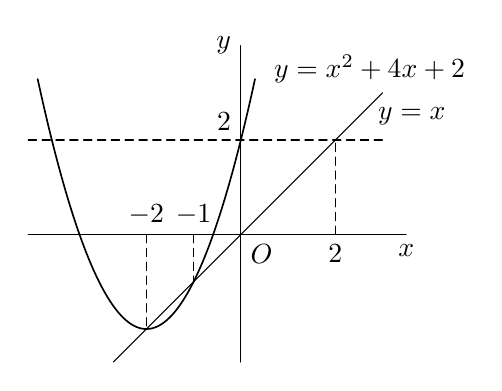
\begin{tikzpicture}[line cap=round,line join=round,scale=0.6]
      \draw[\myaxisarrow] (-4.5,0) -- (3.5,0) node[below] {$x$};
      \draw[\myaxisarrow] (0,-2.7) -- (0,4) node[left] {$y$};
      \draw[line width=0.6pt,smooth,samples=100] 
        plot[domain=-4.3:0.3](\x,{(\x)^2+4*(\x)+2});
      \draw[densely dashed] (-4.5,2)--(3,2) (2,0) node[below] {$2$}--(2,2)
        (-2,0) node[above] {$-2$}--(-2,-2)
        (-1,0) node[above] {$-1$}--(-1,-1);
      \draw (0,0) node[anchor=north west] {$O$}
        (0,2) node[anchor=south east] {$2$} (-2.7,-2.7)--(3,3)
        (0.5,3.5) node[right] {$y=x^2+4x+2$}
        (2.7,2.5) node[right] {$y=x$};
    \end{tikzpicture}
  \end{figure}
  \endsolution
  
  \begin{exercise}
    若函数 $f(x)=a^x -x-a$ ($a>0$ 且 $a\neq1$) 有两个零点,
    求实数 $a$ 的取值范围.
  \end{exercise}

  \beginsolution
    分 $0<a<1$ 和 $a>1$ 讨论, 作图知 $a\in(1,+\infty)$.
  \endsolution
  
  \begin{exercise}
    已知关于 $x$ 的二次方程 $x^2 +2mx+2m+1=0$.
    
    (1) 若其两根分别在区间 $(-1,0)$ 和 $(1,2)$ 内,
    求实数 $m$ 的取值范围;
    
    (2) 若该方程的两根均在区间 $(0,1)$ 内, 求实数 $m$ 的取值范围.
  \end{exercise}
  
  \beginsolution
    设 $f(x)=x^2 +2mx+2m+1$,
    
    (1) 由图象可知
    \[f(-1)>0,\quad f(0)<0,\quad f(1)<0,\quad f(2)>0,\]
    解得 $m\in\Bigl(-\frac52,-\frac12\Bigr)$.
    
    (2) 仍由图象可知
    \[\text{轴 }x=-m\in(0,1),\quad f(-m)<0,\quad f(0)>0,\quad f(1)>0,\]
    解得 $m\in\Bigl(-1,-\frac12\Bigr)$.
  \endsolution

  \begin{exercise}
    若关于 $x$ 的方程 $a^x=x^2$ ($a>1$) 恰有两根, 求 $a$ 的值.
  \end{exercise}

  \beginsolution
    作图知, $a^x=x^2$ 在 $(-\infty,0]$ 上恰有一根, 故在 $(0,+\infty)$ 上也恰有一根, 此时方程化为 $x\ln a=2\ln x$, 表明函数 $f(x)=x\ln a$ 与 $g(x)=2\ln x$ 的图象相切. 设切点横坐标为 $x_0$, 则
    \[\left\{\begin{array}{ll}
        f(x_0)=g(x_0),\\ f'(x_0)=g'(x_0),
      \end{array}\right.\text{\ 即\ }\quad
      \left\{\begin{array}{ll}
        x_0\ln a=2\ln x_0,\\ \ln a= \frac2{x_0},
      \end{array}\right.\]
    则 $x_0=\mathrm{e}$, $a=\mathrm{e}^{\frac2{x_0}}= \mathrm{e}^{\frac2{\mathrm{e}}}$.
    
    \varexercise 题中 ``$a>1$'' 改为 ``$a>0$'', 求 $a$ 的值.
    
    显然 $a=1$ 合题意, 而当 $a>1$ 时已有 $a=\mathrm{e}^{\frac2{\mathrm{e}}}$. 当 $0<a<1$, 方程改写为 $\Bigl(\frac1a\Bigr)^{-x}=(-x)^2$, 故利用已有结论知
    \[\frac1a= \mathrm{e}^{\frac2{\mathrm{e}}}, \text{\ 即\ }
      a=\mathrm{e}^{-\frac2{\mathrm{e}}}.\]
    综上知, $a=\mathrm{e}^{-\frac2{\mathrm{e}}}$,$1$,$\mathrm{e}^{\frac2{\mathrm{e}}}$.
  \endsolution
  
%%%%%%%%%%%%%%%%%%%%%%%%%%%%%%%%%%%%%%